For a real world recognition task, an algorithm that can continuously adaptive to new labels just like the human does, is always very attractive and practical.
In this section, we propose an adaptive method for learning new categories with a few target examples using the feature representations from GoogLeNet. By warm start the parameters of the classifiers, our method can effectively learning new categories. The experiment results show that our method is able to adapt new categories with just a few examples and outperforms the method that learning directly with a large margin.
For the rest part of this section, we first discuss the limitation of some previous domain adaptation approaches for our task, then we introduce our method and show the improved performance on the same task.

%To illustrate our method, we design the following experiment, transferring from Food-101 dataset to Food-256 dataset while just using a few examples. Since Food-101 has more images per category, we use it as the source domain and the fine-tuned GoogLeNet on Food-101 from Section \ref{sec:ft} is used as the feature extractor to generate feature representations for both datasets.
%
%Food-101 and Food-256 datasets share about 36 categories even though the images in the same category may vary across these two datasets. The types of food in Food-101 are mainly western style while most types of food in Food-256 are typical Asian foods. To make this task more challenging, we also limited the number of examples in both source and target domain. Unlike those previous studies which only consider the performance within the target domain, since the two domains are within the general food domain, we combine these two domains together as a more general super-domain and evaluate the accuracy over all the categories in this super-domain.
%The experiment results show our method is able to adapt new categories and outperforms the method that learning directly with a large margin.
%For the rest part of this section, we first discuss the limitation of some previous domain adaptation approaches for our task, then we introduce our method and show the improved performance on the same task.
\subsection{Limits of previous approaches}
From previous studies, there are two kinds of approach to solve our task. The first approach is to fine-tuning the deep CNN with the target examples incorporating with the sources ones.
Fine-tuning the deep CNN model focuses on learning good feature representations from the images and using linear models for classification. From Section \ref{sec:ft}, we successfully use this approach to transfer the knowledge from a general domain to our food domain with impressive results. Indeed, deep CNN can learn discriminative features effectively and by taking advantage of this, this approach achieved some impressive results from previous studies\cite{Chatfield14} \cite{zeiler2014visualizing}. However, fine-tuning on deep CNN requires an ample amount of labeled target data and sometimes could degrade the performance when the labeled examples are scarce\cite{hoffman2013one}. There are many hyperparameters that affect the performance of deep CNN and fine-tuning it on a sparse label condition can lead to horrible overfitting. Apart from its sensitivity to the hyperparameters, fine-tuning the whole network requires intensive computational resources which makes it inappropriate for online learning.

Rather than learning efficient representations, another typical approach are more focused on dealing with the representation learned from conventional feature extraction methods for domain adaptation.
%Many methods have been proposed by minimizing the representation distance between the source and target domain in an unsupervised manner \cite{gong2012geodesic}\cite{fernando2013unsupervised}.
Supervised domain adaptation models, such as Adaptive-SVM (A-SVM) and PMT-SVM, try to utilize the knowledge from source domain and apply to target domain and hypothesize that there should be a relatively strong relationship between the categories among these two domains\cite{yang2007adapting}\cite{aytar2011tabula}. These methods are limited in our task for the reasons that all these methods try to find the similarity between the source and target domain. Indeed, they work well when these two domains have many overlapped or similar categories. However, sparse representations from deep CNN from which the linear classifiers would eventually benefit indicates that the distance of the representations between different categories could be very large.

From empirical experiments, we find that adaptive methods suffer as the difference of source and target categories increases. Table \ref{tab:su_domian} shows some empirical experiment results for two typical domain adaptation methods in a binary classification scenario. We manually choose the similar/identical source categories for the target ones if possible. For the those categories which we fail to find even similar category in source domain, we just choose the category whose representations are most similar to the target one measured by cosine similarity. The parameters used in these methods are set as the default because we think that tuned the parameters for these methods won't improve the performance very much for this experiment.  From the result of our simple experiment, we can see that A-SVM and PMT-SVM suffers from choosing the appropriate domain categories for new categories in target domain. And for our task which is a multi-class situation and more complicated than this, the performance of these methods could be worse than training without any of these adaptive methods.
% Table generated by Excel2LaTeX from sheet 'Sheet1'
\begin{table*}[htbp]
  \centering
  \caption{Average Precision for A-SVM, PMT-SVM, SVM and Logistic Regression. Source categories without * are determined by cosine similarity}
    \begin{tabular}{cccccc}
    \toprule
    Category from food 256 & Category from food 101 & A-SVM  & PMT-SVM & SVM &LR\\
    \midrule
%    Green salad & Caesar salad & 0.1627 & 0.1622 \\
    Doughnut & Doughnut & 0.4771 & 0.4735 &0.4781&0.4554\\
    Caesar salad &  Caesar salad & 0.9488 & 0.9496 &0.9498&0.9486\\
    White rice  & Fried rice & 0.8118 & 0.7932 &0.7932&0.9004\\
    Oatmeal & French onion soup* & 0.0345 & 0.0381 & 0.0347 &0.0454\\
    Pork cutlet & French fries* & 0.0446 & 0.0381 &0.0450& 0.0837\\
    \bottomrule
    \end{tabular}%
  \label{tab:su_domian}%
\end{table*}%

As far as we know, few study has shown that there is an approach that can solve our task. Therefore, we propose an incremental adaptive learning algorithm to solve this problem.
\subsection{Incremental adaptive learning for new category}
Chu et al. recently proposed a warm start approach for parameter selection in linear model and by iteratively updating the parameters optimized from previous knowledge and their algorithm can search the optimal value for a specific task\cite{chuwarm}. Inspired by this, we propose a warm start adaptive learning algorithm that can adapt new categories from the target domain in an incremental learning mode. Instead of learning the whole target categories directly, our method adapts one category each time and iteratively updates all the parameters.
Our method uses logistic regression to classify the representations obtained from deep CNN since compared to deep models, linear model can be more easily trained with just a few examples in each category.
For learning a new category, rather than utilizing the parameters from source domain, we employ another negative binary classifier pre-trained with all the examples from other categories as the negative class and warm start the classifier with the parameters of the negative classifier for the new category. This approach can be extended into an incremental domain adaptation scenario when the algorithm just adapts one category in each step for multi-class situation. For each step, considering $M$ categories in the source domain $S$ and a new category $t$ from target domain $T$, there are $M$ binary classifiers $F=\left\{ {{f}\left( {{w_i},{b_i}} \right)} \right\}_{i = 1}^M$ for each category in $S$ and the negative classifier $\hat{f}=f(\hat{w},\hat{b})$ using all the examples in $\mathcal{P^-}=S$ as negative examples. The classifier $f_t$ for the new category $t$ is initialized with $\left\{\hat{w},\hat{b}\right\}$ and trained with $\mathcal{P^-}\bigcup\mathcal{P^+}$ while $\mathcal{P^+}=t$. Then we update the negative classifier $\hat{f}$ with negative examples $\mathcal{P^-}=S\bigcup t$. The complete strategy for our method is given in Algorithm \ref{algo:ws}.
\begin{algorithm}
  \caption{Complete algorithm of warm start adaptation}\label{algo:ws}
  \begin{algorithmic}[1]
    \REQUIRE Source domain $S = \{ {s_i}|i = 1,..M\} $, Target domain $T = \{ {t_j}|j = 1,..N\} $, Classifier $F = \{\emptyset\}$
    \ENSURE $F$\\
    \FORALL {$i\in M$}
         \STATE $\mathcal{P^+}\leftarrow s_i, \mathcal{P^-}\leftarrow S-s_i$\\
          Train ${{f_i}\left( {{w_i},{b_i}} \right)}$ with $\mathcal{P^+}\bigcup\mathcal{P^-}$, $F\leftarrow F\bigcup f_i$
    \ENDFOR
    \STATE Training negative $\hat{f}\left( {\hat{w_i},\hat{b_i}} \right)$ with $\mathcal{P^-}=S$
    \WHILE {$t_j  \notin S$}
         \FORALL {$i\in M$}
             \STATE $\mathcal{P^+}\leftarrow s_i, \mathcal{P^-}\leftarrow S-s_i+t_j$ \\
              Update ${{f_i}\left( {{w_i},{b_i}} \right)}$ with $\mathcal{P^+}\bigcup\mathcal{P^-}$
        \ENDFOR
        \STATE Initialize $f_j$ with $(\hat{w},\hat{b})$ and train with .
        \STATE $F\leftarrow\ F\bigcup f_j$
        \STATE $S\leftarrow S\bigcup t_j, M\leftarrow M+1$
        \STATE Update $\hat{f}$ with $\mathcal{P^-}=S+t_j$
     \ENDWHILE
  \end{algorithmic}
\end{algorithm}
In our task, compared to those methods using the previous parameters directly, the warm start can start with a better initialization for the new category and thus can be more adaptive for new categories. We use Stochastic Gradient Descent (SGD) to update the parameters for all the binary classifiers as well as the negative classifier.
\begin{figure*}
  \centering
  % Requires \usepackage{graphicx}
  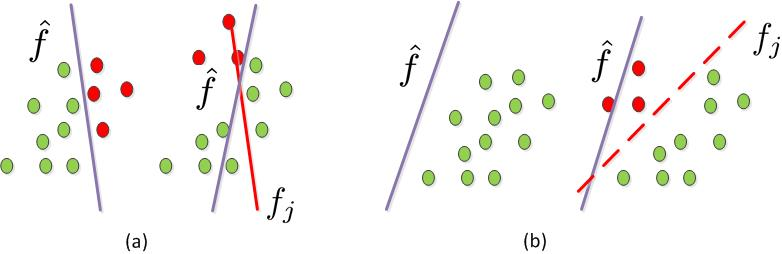
\includegraphics[scale = .6]{fig/domain.jpg}\\
  \caption{(a) Conventional adaptation method fail to find good initialization for the new category from source domain. (b) The parameters from $\hat{f}$ are more adaptive for the new categories.}
  \label{fig:wm}
\end{figure*}

\subsection{Experiment setup \& Evaluation}
To illustrate our method, we design the following experiment, transferring from Food-101 dataset to Food-256 dataset while just using a few examples. Since Food-101 has more images per category, we use it as the source domain and the fine-tuned GoogLeNet on Food-101 from Section \ref{sec:ft} is used as the feature extractor to generate feature representations for both datasets and deep feature representations from \emph{Pool5}, the layer before auxiliary linear classifier, are used as the inputs of our method.

The types of food in Food-101 are mainly western style while most types of food in Food-256 are typical Asian foods. They share about 36 categories even though the images in the same category may vary across these two datasets. These 36 duplicated categories are removed as noisy categories, so there are 220 new categories left in Food-256 dataset.
To make this task more challenging, we also limited the number of examples in both source and target domain.

Baseline: Instead of using the supervised adaptation techniques, such as A-SVM, we use cold start which randomly initializes the parameters for all the classifiers, as our baseline, because from Table \ref{tab:su_domian} we can see when adapting new categories, SVM and LR without any adaptation technique show similar results to those adaptive methods. The hypothesis of these adaptive methods limits their ability to adapt new categories as we discuss above.

\emph{n shorts:} In our experiments, the training set of $n$ shots contains $n$ randomly picked examples from each category in both Food-101 and Food-256 datasets and the test set contains all the rest examples in Food-256 only.

For our SGD, we use effective learn rate following polynomial decay, to be 0 at max iteration and set base learning rate to 0.01. The initialization of the classifiers for source domain are trained with all the examples from source domain and negative classifier are initialized the same way as well. Unlike the other studies which consider the performance within the target domain separately, since the categories in our two datasets are in the general food category we would rather considering to combine them together as a super-domain and evaluate the performance for target categories on this super-domain.
\subsection{From 101 to 102 categories}
When there are multiple categories in target domain, our method divides the learning procedure into several steps and adapts one category in each step, updating all the parameters of the binary logistic regression classifiers. So for the experiment adapting Food-256 from Food-101, the algorithm starts from a 101 to 102 categories situation. We conduct the following experiment: we try to add an arbitrary category from Food-256 to Food-101 and evaluate accuracy of the new category in the super-domain containing 102 categories. We go through all the 220 categories in Food-256 in each round and Table \ref{tab:N+1} shows the average performance of 10 rounds experiments.

\begin{table}[htbp]
  \centering
  \caption{Accuracy for a single new target category in M+1 experiment. Average top-5 accuracies for some categories are shown. Last row shows the average results for all categories.}
    \begin{tabular}{c|cc|cc}
    \toprule
          & \multicolumn{2}{c|}{5 shots} & \multicolumn{2}{c}{1 shot} \\
    \midrule
       target category   & \multicolumn{1}{c}{Warm} & \multicolumn{1}{c|}{Cold} & \multicolumn{1}{c}{Warm} & \multicolumn{1}{c}{Cold} \\
        \midrule
    crape & \textbf{84.16} & 62.29 & \textbf{56.20}  & 28.00 \\
   chip butty & \textbf{80.97} & 65.82 & \textbf{55.03} & 37.40 \\
    meat loaf & \textbf{67.78} & 53.15 & \textbf{68.21} & 56.07 \\
    dried fish & \textbf{92.00}    & 79.81 &\textbf{83.85} & 71.19 \\
   scrambled egg & \textbf{75.21} & 63.54 & \textbf{59.00}    & 43.20 \\
    pork belly & \textbf{81.76 }& 70.59 &\textbf{53.21} & 32.45 \\
%    natto & 79.01&\textbf{80.70}&\textbf{73.69}&66.71\\
%    miso soup &\textbf{96.06}&95.92&91.04&\textbf{94.52}\\
    \midrule
    %Average &\textbf{91.91$\pm$8.15}&88.82$\pm$10.40  & \textbf{80.77$\pm$ 12.03} & $71.78\pm 15.07 $ \\
    Overall average &\textbf{91.91}&88.82  & \textbf{80.77} & 71.78 \\
    \bottomrule
    \end{tabular}%
  \label{tab:N+1}%
\end{table}%
From Table \ref{tab:N+1} we can see that by taking advantage of the warm start, the warm start does a slightly better than cold start in M+1 experiment since the initialization difference between these two methods are too small. We believe the margin of these two methods would increase as more new categories are learned from warm start.
%%%%%%%%%%%%%%%%%%%%%%%%%%%%%%%%%%%%%%%%%%%%%%%%%%%%%%%%%%%%%%%%%%%

\subsection{From 101 to 101+220 categories}
In this part, we show the performance of warm start in multiple new categories situation. From the experiments above, warm start shows some improvement on cold start and experiment shows that the improvement can be accumulated as more categories are learned. Because the parameters of the negative classifier can affect the whole procedure greatly and randomly picking only one example from each category can be significantly bias, we fail to get a convergent result for both warm and cold starts in one short experiment.
From empirical experiments we find that in order to get a convergent result, we have to pick at least 5 examples in each category. So we only show the performance of five shots for this experiment. In each step, the new category is determined by its original class index in Food-256. We use run SGD 50 iterations for each step and run this experiment 10 times as well. Figure \ref{fig:wama} shows the average results in 5 short for both warm and cold start in each step.

\begin{figure*}
  \centering
    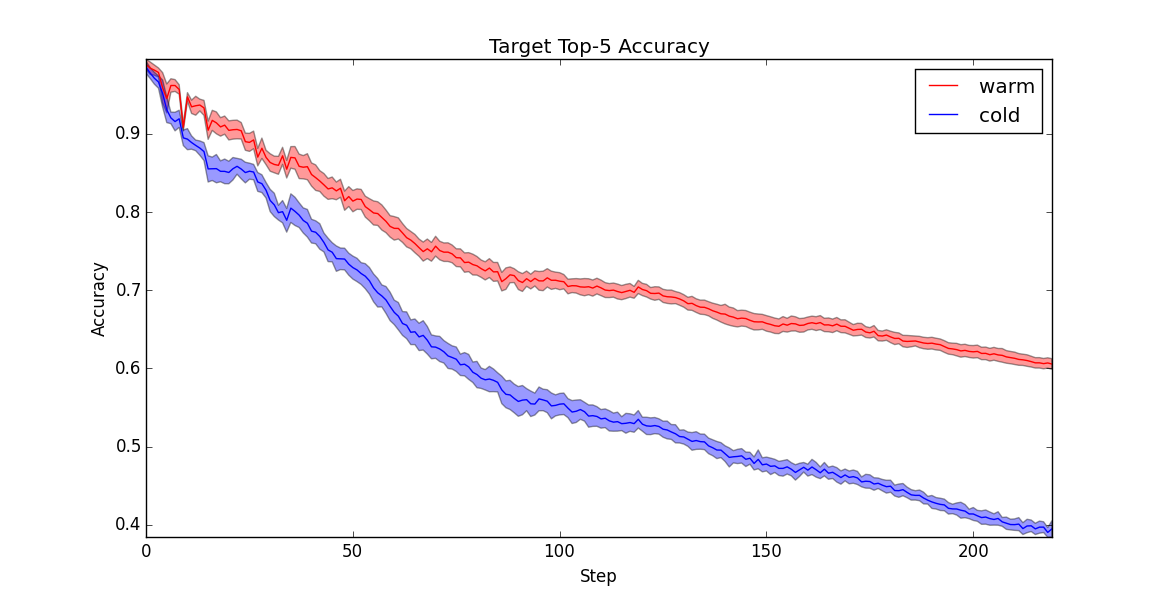
\includegraphics[scale=0.4]{fig/M+N.png}
    \caption{Top-5 accuracy curve for categories in Food-256 in super-domain with 5 shots. Mean and standard deviation are shown.}
      \label{fig:wama}
\end{figure*}

From Figure \ref{fig:wama} we can see that benefitting from warm start, classifiers can accumulate the information from previous steps and thus the margin between warm and cold starts increases as more new categories are learned. Indeed, cold start may not converge well for just 50 iterations. We believe that given enough training iteration, warm start can still converge to a better result (see Figure \ref{fig:errdiff}). We compare the results for different iterations and the average performance of 10 experiments are shown in Table \ref{tab:it}. The results of cold start in 10 and 20 iterations experiments, which are not even significantly better than random guess, are ignored. We observe that increasing training iteration won't help improve the performance of warm start very much as it converges very fast by taking advantage of better initialization.
\begin{figure*}[htbp]
\centering
\subfigure{
    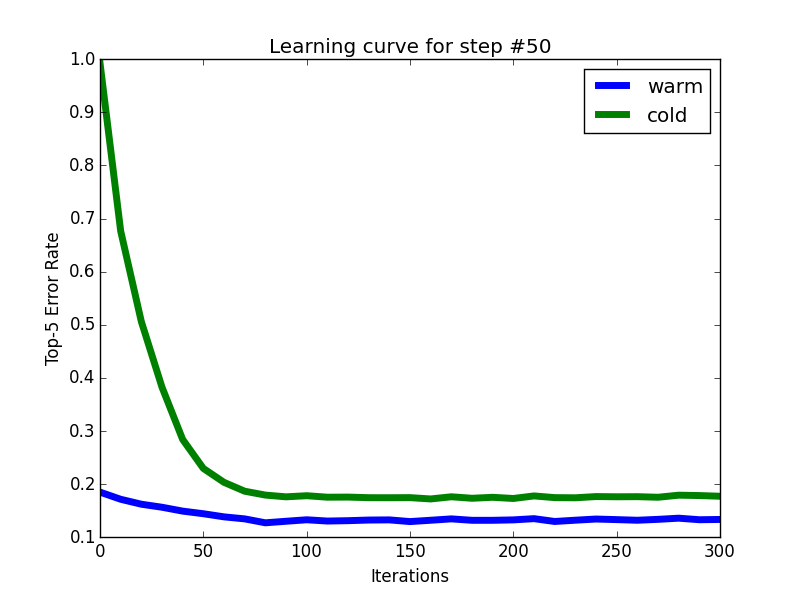
\includegraphics[width=0.3\textwidth]{fig/50W.png}
}
\subfigure{
    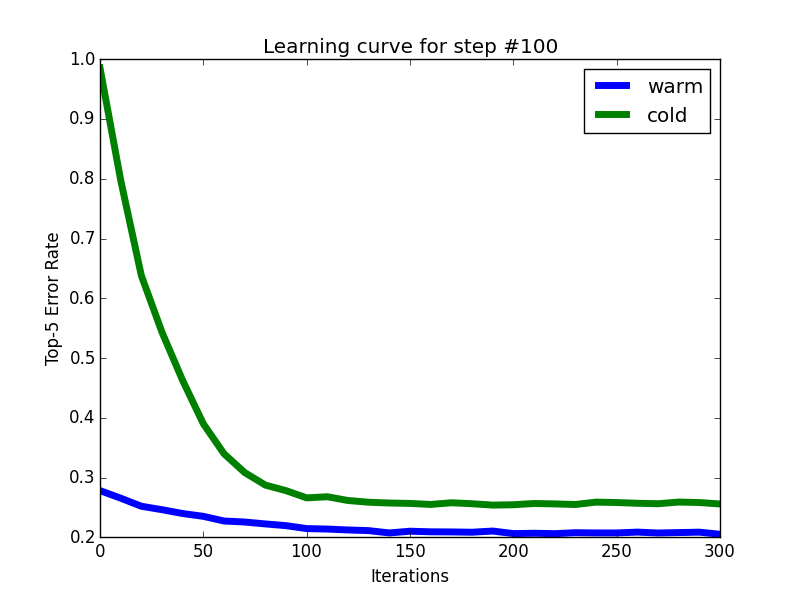
\includegraphics[width=0.3\textwidth]{fig/100W.png}
}\\
\subfigure{
    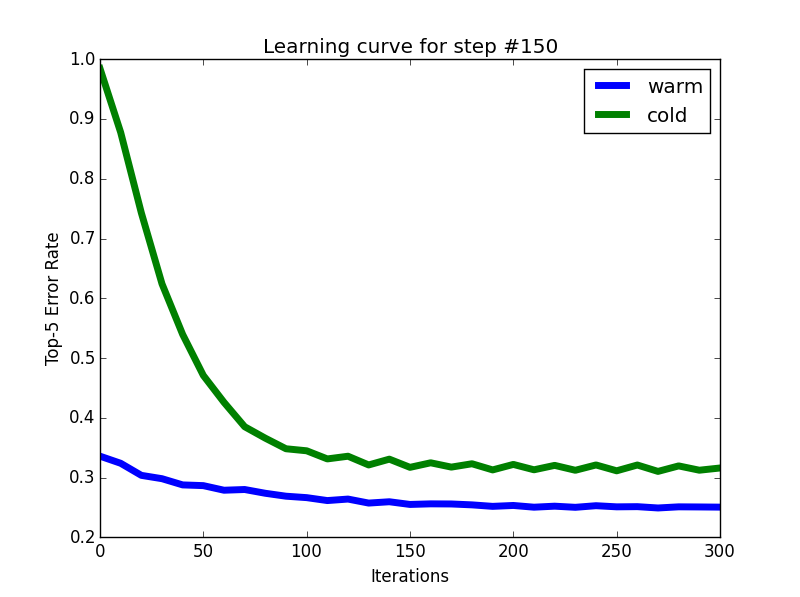
\includegraphics[width=0.3\textwidth]{fig/150W.png}
}
\subfigure{
    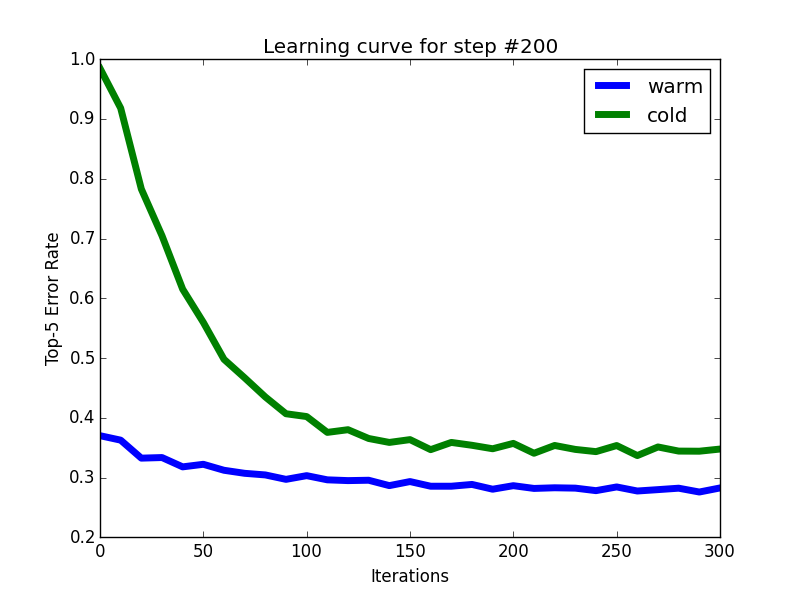
\includegraphics[width=0.3\textwidth]{fig/200W.png}
}
\caption{Overall learning curve in some steps for 300 iterations. \textbf{Observation:} even training with enough iteration, warm start can still outperform cold start in a single step.}
\label{fig:errdiff}
\end{figure*}
% Table generated by Excel2LaTeX from sheet 'Sheet1'
\begin{table*}[htbp]
  \centering
  \caption{Top-5 accuracy for 220 new categories in super-domain with different training iteration in each step.}
    \begin{tabular}{C{1cm}c|c|cc|cc}
    \toprule
          & 10 iterations&20 iterations &\multicolumn{2}{c|}{50 Iterations} & \multicolumn{2}{c}{300 iterations} \\
    \midrule
          & warm start & warm start& warm start & cold start & warm start & cold start \\
    Top-5& 60.37$\pm$ 0.58   &    60.54$\pm0.32$  &60.33$\pm$0.62   &     39.10$\pm$0.66   &    \textbf{61.48$\pm$0.59 }  & 55.35$\pm$0.48 \\
    \bottomrule
    \end{tabular}%
  \label{tab:it}%
\end{table*}%
